%% LaTeX Beamer presentation template (requires beamer package)
%% see http://bitbucket.org/rivanvx/beamer/wiki/Home
%% idea contributed by H. Turgut Uyar
%% template based on a template by Till Tantau
%% this template is still evolving - it might differ in future releases!

\documentclass{beamer}

\mode<presentation>
{
\usetheme{Warsaw}

\setbeamercovered{transparent}
}

\usepackage{../../Common/sty/TI84} %TODO: How to get the link working...?



\title{Masterclass programmeren op de GR TI-84 (les 4)}

%\subtitle{}

% - Use the \inst{?} command only if the authors have different
%   affiliation.
%\author{F.~Author\inst{1} \and S.~Another\inst{2}}
\author{Kevin van As}

% - Use the \inst command only if there are several affiliations.
% - Keep it simple, no one is interested in your street address.
% \institute[Universities of]
% {
% \inst{1}%
% Department of Computer Science\\
% Univ of S
% \and
% \inst{2}%
% Department of Theoretical Philosophy\\
% Univ of E}

\date{\today}


% This is only inserted into the PDF information catalog. Can be left
% out.
\subject{Masterclass GR TI-84 programmeren (les 4)}



% If you have a file called "university-logo-filename.xxx", where xxx
% is a graphic format that can be processed by latex or pdflatex,
% resp., then you can add a logo as follows:

% \pgfdeclareimage[height=0.5cm]{university-logo}{university-logo-filename}
% \logo{\pgfuseimage{university-logo}}



% Delete this, if you do not want the table of contents to pop up at
% the beginning of each subsection:
\AtBeginSubsection[]
{
\begin{frame}<beamer>
\frametitle{Outline}
\tableofcontents[currentsection,currentsubsection]
\end{frame}
}

% If you wish to uncover everything in a step-wise fashion, uncomment
% the following command:

%\beamerdefaultoverlayspecification{<+->}

\begin{document}

\begin{frame}
\titlepage
\end{frame}


\begin{frame}
\frametitle{Recap!}

% \visible<2>{\ticalcfig{\ticalcfigCircle{\ticalcfigCircleColThree}{0.615}}} % prgm
% \visible<3-4>{\ticalcfig{\ticalcfigCircle{\ticalcfigCircleColFour}{0.62}}} % Vars
% \visible<5>{\ticalcfig{\ticalcfigCircle{\ticalcfigCircleColThree}{0.615}}} % prgm

We hebben gekeken naar:
\begin{itemize}
	\item<2-> Herhaling / Repetitie
		\begin{itemize}
		  \item<3-> Goto \& Labels
		  \item<4-> For-loops
		  \item<5-> While-loops
		\end{itemize}
	\item<6-> Pause
	\item<7-> Datatype: Lists
\end{itemize}
\end{frame}

\begin{frame}
\frametitle{Vooruitzicht!}

Vandaag zullen we kijken naar:
\begin{itemize}
	\item<2-> Advanced I/O:
		\begin{itemize}
		  \item<3-> Menu
		  \item<4-> Output
		  \item<5-> ClrHome
		\end{itemize}
	\item<6-> Custom functions
	\item<7-> Tips 'n Tricks:
		\begin{itemize}
		  \item<8-> \tiCLEAR\,om een menu te sluiten
		  \item<9-> \tiALPHA-scrolling
		  \item<10-> \tiCATALOG
		  \item<11-> Debugging
		  \item<12-> Afrondingsfouten
		\end{itemize}
\end{itemize}

\end{frame}


%% END %%

\begin{frame}
\frametitle{Outline}
\tableofcontents
% You might wish to add the option [pausesections]
\end{frame}

% The core pages
\section{Tips 'n Tricks}

\subsection{Random tips}

\begin{frame}
\frametitle{Trial 'n Error}

\begin{itemize}
  \item<1-> Soms is het lastig om te beredeneren of er nu \tifonttxt{A+1\>A} moet staan, of juist \tifonttxt{A-1\>A}.
  \item<2-> Of is de juiste initialisatie nou \tifonttxt{\min 1\>A} of \tifonttxt{0\>A}?
  \item<3-> In dit soort gevallen kan de ``Trial 'n Error'' tactiek nuttig zijn:
  \begin{itemize}
    \item<4-> ``Probeer gewoon wat, en zie wat er gebeurt!''
    \item<5-> W\'e\'et wat de uitkomst van je \tifonttxt{prgm} moet zijn, en corrigeer de code indien het resultaat niet klopt.
  \end{itemize}
  \item<6-> Let wel: Test genoeg cases om zeker te weten dat je \tifonttxt{prgm} nu klopt!
    Immers, je hebt je code `gegokt', niet bedacht.
\end{itemize}

\end{frame}



\begin{frame}
\frametitle{\tiCLEAR\,om een menu te sluiten}

\only<1-2>{\ticalcfig{\ticalcfigCircle{\ticalcfigCircleColTwo}{0.805}}}
\only<3->{\ticalcfig{\ticalcfigCircle{\ticalcfigCircleColFive}{0.636}}}

\begin{itemize}
  \item<1-> \lenitem{Ik heb altijd de neiging om \tiSecond\tiMODE=\tiQUIT\,te gebruiken om een menu te sluiten.}
  \item<2-> \lenitem{Klinkt logisch, maar indien je dit doet in een \tifonttxt{prgm},
    dan sluit je zowel het menu als het \tifonttxt{prgm} en moet je je \tifonttxt{prgm} weer overnieuw openen\ldots}
  \item<3-> De correcte manier om een menu te sluiten is daarom dus ook de \tiCLEAR-knop. Dit sluit elk menu, maar sluit niet je \tifonttxt{prgm}.
  \item<4-> Let wel: clear niet per ongeluk een regel van je \tifonttxt{prgm} door 2x te drukken op \tiCLEAR.
\end{itemize}

\end{frame}




\begin{frame}
\frametitle{\tiALPHA-scrolling}


\only<1>{\ticalcfig{\ticalcfigCircleDown}}
\only<2>{\ticalcfig{\ticalcfigCircleAlpha\ticalcfigCircleDown}}
\only<3>{\ticalcfig{\ticalcfigCircleSecond\ticalcfigCircleAlpha}}

\begin{itemize}
  \item<1-> \lenitem{Naarmate je \tifonttxt{prgm} langer wordt, wordt het vervelender om door je \tifonttxt{prgm} te navigeren.}
  \item<2-> \lenitem{Door \tiALPHA\tiDown\,te gebruiken i.p.v. \tiDown\,, scroll je significant sneller.}
  \item<3-> Met behulp van \tiSecond\tiALPHA=\tiALOCK\,, kun je herhaaldelijk snel scrollen. Try it yourself!
\end{itemize}

\end{frame}




\begin{frame}
\frametitle{Meet your new best friend: Google}

\begin{itemize}
  \item<1-> Whenever you run into a problem, someone else has most certainly had the same problem.
  \item<2-> Therefore, your problem has already been solved before.
  \item<3-> So, when you want to do something, but you do not know how to do it, you ask your best friend.
  \item<4-> Note: The internet is English (like this slide). So use English search terms for the best result.
\end{itemize}


\end{frame}



\begin{frame}
\frametitle{Vooral veel commentaar leveren}

\begin{itemize}
  \item<1-> Het is handig om ``comments'' in je code achter te laten.
  \item<2-> Dit zijn kleine notes die uitleggen wat je code doet.
  \item<3-> Indien je later weer naar je code kijkt, helpen die je begrijpen wat je code doet.
  \item<4-> Dit kun je met behulp van een string doen: \inlineticalc{\qt COMMENT}
  \item<5-> WARNING: Dit overschrijft de waarde van \tifonttxt{Ans}!
\end{itemize}

\vspace{1.5cm}

\begin{tikzpicture}[overlay,remember picture]
	\node[yshift=0.6cm] (BL) at (current page.south east){ };
	\node [anchor=south east,xshift=0.195cm] (BL2) at (BL)
	{%
	\only<4>{%
		\begin{ticalc}[5cm]
			PROGRAM\:ABC\\%
			\:\qt SOLVE\,AX\sq+BX+C=0\\%
			\:Prompt\,A\comma B\comma C\\%
			\:B\sq-4AC\>D\\%
			\:Disp (\min B+\sqrt(D))/(2A)\\%
			\:Disp (\min B-\sqrt(D))/(2A)
		\end{ticalc}
	}%
	\only<5->{%
		\begin{ticalc}[5cm]
			PROGRAM\:ABC\\%
			\:Prompt\,A\comma B\comma C\\%
			\:\qt SOLVE\,AX\sq+BX+C=0\\%
			\:B\sq-4AC\>D\\%
			\:Disp (\min B+\sqrt(D))/(2A)\\%
			\:Disp (\min B-\sqrt(D))/(2A)
		\end{ticalc}
	}%
	};
\end{tikzpicture}


\end{frame}







\subsection{Debugging}

\begin{frame}
\frametitle{Wat is ``debugging''?}

\begin{itemize}
  \item<1-> Wat is een `bug'?
  \begin{itemize}
    \item<2-> Wikipedia: ``A software bug is an error, flaw, failure, or fault in a computer program or system
      that causes it to produce an incorrect or unexpected result, or to behave in unintended ways.''
    \item<3-> Oftewel, je \tifonttxt{prgm} doet niet wat je wilt.
  \end{itemize}
  \item<4-> Waar komen die beesten vandaan?
  \begin{itemize}
    \item<5-> Wikipedia: ``Most bugs arise from mistakes and errors made by people in either a program's source code or its design.''
    \item<6-> Oftewel, een programmeer- of denkfout.
  \end{itemize}
  \item<7-> Debugging is ``het verwijderen van bugs''
  \item<8-> Indien je de `Trial 'n Error' tactiek gebruikt, dan maak je met opzet bugs om ze vervolgens gelijk te verwijderen.
\end{itemize}


\begin{tikzpicture}[overlay,remember picture]
	\node[] (BL) at (current page.south east){ };
	\node [anchor=south east,yshift=0.6cm] at (BL)
	{%
	\only<1-4>{
\includegraphics[height=0.45\textheight]{../figures/bugs.png}}
	\only<5-7>{
\includegraphics[height=0.28\textheight]{../figures/bugs.png}}
	};
\end{tikzpicture}

\end{frame}



\begin{frame}
\frametitle{Hoe kun je debuggen?}

\begin{itemize}
  \item<1-> Test je \tifonttxt{prgm} vaak, en negeer onverwachtte resultaten niet: als iets \'e\'en keer gebeurt, dan zal het vaker gebeuren.
  \item<2-> Traceer stap voor stap:
  \begin{itemize}
    \item<3-> welke input waardes tot het probleem leiden \tifonttxt{\>} test cases.
	\item<4-> waar in je \tifonttxt{prgm} alles nog klopt {\tiny{(zie volgende slide)}}, en waarna er iets mis gaat = onverwachtte waardes.
  \end{itemize}
  \item<5-> Het helpt om het \tifonttxt{prgm} zelf (in je hoofd - brain power) uit te voeren. Doet je rekenmachine hetzelfde als jij met de hand doet?
    Zo niet, dan werkt een functie anders dan je dacht.
\end{itemize}

\vspace{2cm}

\begin{tikzpicture}[overlay,remember picture]
	\node[] (BL) at (current page.south east){ };
	\node [anchor=south east,yshift=0.6cm] at (BL)
	{%
	\only<1->{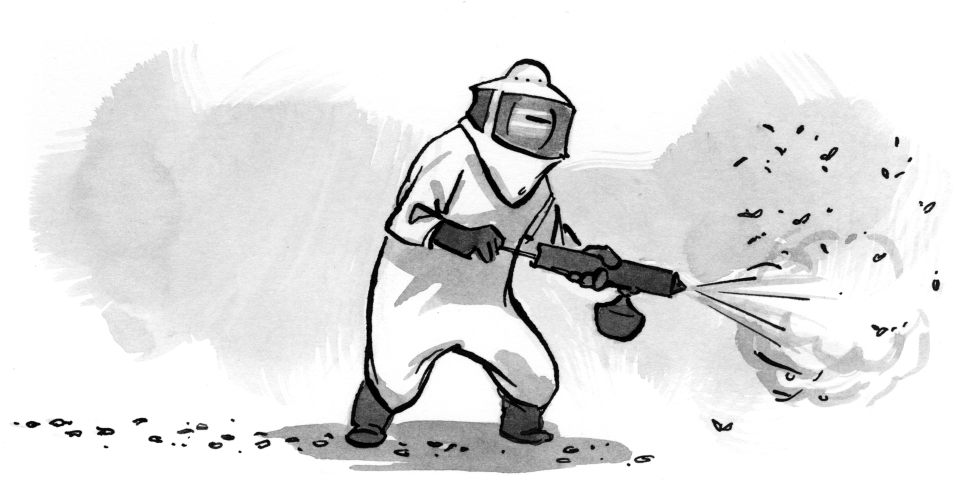
\includegraphics[height=0.28\textheight]{../figures/debugging.jpg}}
	};
\end{tikzpicture}

\end{frame}



\begin{frame}
\frametitle{\tifonttxt{Pause} statement: Localiseer de bug}

\visible<3>{\ticalcfig{\ticalcfigCircle{\ticalcfigCircleColOne}{0.128}}} % ON button

\vspace{-1cm}
\hspace{-1cm}
\begin{minipage}{\textwidth}
\begin{itemize}
  \item<1-> \lenitem[0.9\linewidth]{Om een bug te localiseren (=vinden waar in je \tifonttxt{prgm} de fout zit), is het handig om \inlineticalc{Pause} te gebruiken.}
  \item<2-> \lenitem[0.9\linewidth]{Zo kun je je \tifonttxt{prgm} breaken (=middenin zijn executie stoppen) waar je wilt.}
  \item<3-> \lenitem[0.9\linewidth]{Dit doe je door op de \tiON-knop te drukken terwijl je \tifonttxt{prgm} gepauseerd is.}
  \item<4-> Kies dan \tifonttxt{Quit}. (\tifonttxt{Goto} kan ook nuttig zijn - probeer het zelf.)
  \item<5-> Nu kun je alle variabelen bekijken. Is de waarde wat je verwacht had? Zo niet? Dan moet de bug \emph{boven} je \tifonttxt{Pause} statement zitten!
\end{itemize}
\end{minipage}


\begin{tikzpicture}[overlay,remember picture]
	\node[yshift=0.6cm] (BL) at (current page.south east){ };
	\node [anchor=south east,xshift=0.195cm] (BL2) at (BL)
	{%
		\begin{ticalc}
			PROGRAM\:PAUSETST\\%
			\:0\>A\\%
			\:Pause\\%
			\:1\>A
		\end{ticalc}
	};
	\node [anchor=south east,xshift=-3.5cm] (BL3) at (BL)
	{%
		\only<3,5->{%
			\begin{ticalc}%
				prgmPAUSETST\visible<-3>{\pausedots}\\%
				\visible<5->{%
				A\\%
				\hfill 0%
				}%
			\end{ticalc}%
		}%
		\only<4>{%
			\begin{ticalc}%
				ERR\:BREAK\\%
				\select{1\+\:}Quit\\%
				2\:Goto%
			\end{ticalc}%
		}%
	};
\end{tikzpicture}

\end{frame}




\begin{frame}
\frametitle{Example: Debug deze code}

\hspace{-0.8cm}
\begin{minipage}{0.7\textwidth}
Hier is het \tifonttxt{BIRTHDAY} \tifonttxt{prgm} van les 2. Alleen\ldots Ik heb een fout gemaakt! Debug de code m.b.v. test cases.
Bekijk extreme gevallen:

\visible<2->{Wat gebeurt er als ik geboren ben op
\begin{itemize}
  \item 1 Januari 0 en het is 10 Februari 1?
  \only<-5>{\visible<2-5>{\begin{itemize}
    \visible<3-5>{\item \tifonttxt{A=1}}
    \visible<4-5>{\item \tifonttxt{M<N}, dus \tifonttxt{A} blijft \tifonttxt{1}.}
    \visible<5-5>{\item Dat is wat je verwacht: 1 jaar oud.}
  \end{itemize}}}
  \item<6-> 1 Januari 0 en het is 10 Januari 1?
  \only<6-8>{\begin{itemize}
     \visible<6-8>{\item \tifonttxt{A=1}}
     \visible<7-8>{\item \tifonttxt{M=N} en \tifonttxt{E>D}, dus \tifonttxt{A} blijft \tifonttxt{1}.}
     \visible<8-8>{\item Dat is wat je verwacht: 1 jaar oud.}
  \end{itemize}}
  \item<9-> 5 Januari 0 en het is 1 Januari 1?
  \only<9-12>{\begin{itemize}
    \visible<9-12>{\item \tifonttxt{A=1}}
    \visible<10-12>{\item \tifonttxt{M=N} en \tifonttxt{D>E}, dus \tifonttxt{A} wordt \tifonttxt{2}.}
    \visible<11-12>{\item Maar je verwacht \tifonttxt{0} jaar! Een bug!}
    \visible<12-12>{\item Waarschijnlijk moet hier \tifonttxt{A-1\>A} staan!}
  \end{itemize}}
\end{itemize}
}
\end{minipage}
\begin{minipage}{0.28\textwidth}
\begin{ticalc}[3.5cm]
	PROGRAM\:BIRTHDAY\\%
	\:Input\,\qt YOU\,Y\qt\comma Y\\%
	\:Input\,\qt YOU\,M\qt\comma M\\%
	\:Input\,\qt YOU\,D\qt\comma D\\%
	\:Input\,\qt CUR\,Y\qt\comma Z\\%
	\:Input\,\qt CUR\,M\qt\comma N\\%
	\:Input\,\qt CUR\,D\qt\comma E\\%
	\:\\%
	\only<1-2,4-5,7-8,10->{\:Z-Y\>A\\}%
	\only<3,6,9>{\select{\:Z-Y\>A}\\}%
	\:If\,M>N\:Then\\%
	\:A+1\>A\\%
	\:Else\\%
	\only<1-6,8-9,11->{\:If\,M=N\,and\,D>E\\}%
	\only<7,10>{\:If\,\select{M=N\,and\,D>E}\\}%
	\:Then\\%
	\only<1-9>{\:A+1\>A\\}%
	\only<10-12>{\select{\:A+1\>A}\\}%
	\:End\\%
	\:End\\%
	\:Disp\,A
\end{ticalc}
\end{minipage}


\end{frame}






\subsection{Catalog \& CatalogHelp}

\begin{frame}
\frametitle{De bibliotheek}

\only<1-2>{\ticalcfig{\ticalcfigCircle{\ticalcfigCircleColTwo}{0.053}}} % Catalog
\only<3-4>{\ticalcfig{\ticalcfigCircle{\ticalcfigCircleColTwo}{0.628}}} % Apps
\only<5>{\ticalcfig{\ticalcfigCircle{\ticalcfigCircleColOne}{0.64}}} % math menu
\only<6->{\ticalcfig{\ticalcfigCircle{\ticalcfigCircleColFive}{0.225}}} % +

\hspace{-1cm}
\vspace{2cm}
\begin{minipage}{\textwidth}
\begin{itemize}
  \item<1-> \lenitem[0.9\linewidth]{\textbf{Alle} functies van de rekenmachine staan alfabetisch in de catalogus: \tiSecond\tiZero=\tiCATALOG.}
  \item<2-> \lenitem[0.9\linewidth]{Dit zijn \textbf{meer functies} dan in de menus staan!\\ Check it out yourself!}
  \item<3-> \lenitem[0.9\linewidth]{Een nuttige app (\tiAPPS) is \tifonttxt{CtlgHelp}.}\\%
    {\footnotesize{(Download van het internet, of link met iemand die hem heeft.)}}
  \begin{itemize}
    \item<4-> Voer de app uit. De hulpfunctie is nu actief.
    \item<5-> Blader naar een functie naar keuze.\\
      Bijvoorbeeld \tifonttxt{randInt(}.
    \item<6-> Druk nu op \tiPlus\,voor hulp.
    \item<7-> \lenitem[0.7\linewidth]{Je ziet nu de argumenten van de \tifonttxt{randInt(}-functie: wat de GR van je verwacht.}
    \item<8-> \lenitem[0.7\linewidth]{Alles tussen blokhaken (\tifonttxt{[]}) is optioneel (=niet verplicht).}
  \end{itemize}
\end{itemize}
\end{minipage}



\begin{tikzpicture}[overlay,remember picture]
	\node[yshift=0.6cm] (BL) at (current page.south east){ };
	\node [anchor=south east,xshift=0.195cm] at (BL)
	{%
	\only<1>{%
		\begin{ticalc}
			CATALOG\\%
			\ftriangleright abs(\\%
			\,and\\%
			\,angle(\\%
			\,ANOVA(\\%
			\,Ans\\%
			\,Archive\\%
			\,Asm(
		\end{ticalc}
	}%
	\only<2>{%
		\begin{ticalc}
			CATALOG\\%
			\,Get(\\%
			\,GetCalc(\\%
			\ftriangleright getDate\\%
			\,getDtFmt\\%
			\,getDtStr(\\%
			\,getTime\\%
			\,getTmFmt
		\end{ticalc}
	}%
	\only<5>{%
		\begin{ticalc}[3.4cm]
			MATH\,NUM\,CPX\,\select{PRB} \\%
			\one\:rand( \\%
			2\:nPr \\%
			3\:nCr \\%
			4\:! \\%
			\selectitem{5\:}randInt( \\%
			6\:randNorm( \\%
			7\arrowdown randBin(
		\end{ticalc}
	}%
	\only<6->{%
		\begin{ticalc}
			randInt(
			\hline\\%
			(lower\comma upper[\comma nu
			mtrials])\\%
			\hfill\\%
			\hfill\\%
			\hfill\\%
			\hfill\\%
			\hline
		\end{ticalc}
	}%
	};
\end{tikzpicture}

\end{frame}







\subsection{Precisie en afrondingsfouten}

\begin{frame}
\frametitle{Precisie}

\begin{itemize}
  \item<1-> Je rekenmachine slaat \underline{niet} oneindig veel getallen van een rationeel getal op.
  \item<2-> Om precies te zijn, hij slaat 14 getallen op:
\end{itemize}
\visible<2->{
\begin{ticalc}[3.5cm]
	1/9\\%
	\hfill 0.111 111 111 111 11
\end{ticalc}
}
\begin{itemize}
  \item<3-> Dit kan leiden tot afrondingsfouten.
  \item<4-> Zo is \inlineticalc{1/9*9=0.99999999999999\!1}\ldots
  \item<5-> Wat geeft de volgende functie? \visible<6->{\tifonttxt{\>} Niet \tifonttxt{1}, wat je wel wilt\ldots!}
\end{itemize}
\visible<5->{
\begin{ticalc}[3.5cm]
	int(1/9*9)\\%
	\hfill \visible<6->{0}
\end{ticalc}
}

\begin{itemize}
  \item<7-> Gelukkig geeft \inlineticalc{\:If\,1/9*9=1} \underline{wel} gewoon ``true''!
  \item<8-> Enig idee hoe we met afrondingsfouten kunnen omgaan?
\end{itemize}

\end{frame}



\begin{frame}
\frametitle{\tifonttxt{iPart} en \tifonttxt{fPart}}

\visible<2->{\ticalcfig{\ticalcfigCircle{\ticalcfigCircleColOne}{0.635}}} % Math

\begin{itemize}
  \item<1-> Eerst, hoe weet ik dat er 14 getallen zijn?
  \item<2-> Dit kan bewezen worden m.b.v. \tifonttxt{fPart}.
  \item<3-> \lenitem{Dit weergeeft de fraction-part van een getal (alles rechts van de punt).}
  \item<4-> \lenitem{Similarly, \tifonttxt{iPart} is de integer-part (links van de punt).}
\end{itemize}

\begin{itemize}
  \item<5-> \lenitem[0.65\linewidth]{Door de punt te verschuiven, kunnen we tellen hoeveel getallen de rekenmachine op slaat! 14!}
\end{itemize}
		
\vspace{2cm}
		
\begin{tikzpicture}[overlay,remember picture]
	\node[yshift=0.6cm] (BR) at (current page.south east){ };
	\node [anchor=south east,xshift=0.195cm] at (BR)
	{%
	\only<2->{%
		\begin{ticalc}[3.4cm]
			MATH\,\select{NUM}\,CPX\,PRB \\
			\one\:abs( \\
			2\:round( \\
			\selectitem{3\:}iPart( \\
			\selectitem{4\:}fPart( \\
			5\:int( \\
			6\:min( \\
			7\arrowdown max(
		\end{ticalc}
	}%
	};
	\node [anchor=south east,xshift=-3.7cm] at (BR)
	{%
	\only<3-4>{%
		\begin{ticalc}
			fPart(2.5431)\\%
			\hfill 0.5431\\%
			iPart(2.5431)\\%
			\hfill 2
		\end{ticalc}
	}%
	\only<5>{%
		\begin{ticalc}
			fPart(1.2345678 901234567*1\E10)\\%
			\hfill 0.23\selectitem{4}
		\end{ticalc}
	}%
	};
\end{tikzpicture}

\end{frame}






\begin{frame}
\frametitle{Hoe wordt \tifonttxt{1/9*9} weer gelijk aan \tifonttxt{1}?}

\begin{itemize}
  \item Hoe kun je \inlineticalc{\:If\,X=1} aanpassen om met afrondingsfouten om te gaan?
\end{itemize}

\visible<2->{
\begin{itemize}
  \item Dan moeten we een ``ongeveer gelijk aan'' zelf maken\ldots
  \item<3-> Dat kan op veel verschillende manieren! Dit is de makkelijkste:
\end{itemize}

	\visible<3->{
	\begin{ticalc}[10cm]
	\:1/9*9\>X\\%
	\:1\>Y\\%
	\:If\,X/Y+1\E\min9\ge1\,and\,X/Y-1\E\min9\le1\\%
	\:If\,abs(X-Y)+1\E\min9\ge0\,and\,abs(X-Y)-1\E\min9\le0
	\end{ticalc}
	}
	
\begin{itemize}
  \item<4-> Maar \underline{niet} (Waarom?):
\end{itemize}

	\visible<4->{
	\begin{ticalc}[10cm]
	\:If\,X+1\E\min9\ge Y\,and\,X-1\E\min9\le Y\\%
	\end{ticalc}
	}
}


\end{frame}





\begin{frame}
\frametitle{Integer checking}

\begin{itemize}
  \item Wat is een integer (NL: geheel getal)?
\end{itemize}

\visible<2->{
\begin{itemize}
  \item<2-> Een integer heeft een \tifonttxt{fPart} van 0. Dus:
\end{itemize}
\visible<2->{
\begin{ticalc}[3.5cm]
	\:If\,fPart(X)=0\\%
	\:Then\\%
	\:\qt X\,INTEGER\\%
	\:Else\\%
	\:\qt X\,RATIONAL\\%
	\:End
\end{ticalc}
}\visible<4->{
\begin{ticalc}[6cm]
	\:If\,fPart(abs(X)+1\E\min9)<1\E\min7\\%
	\:Then\\%
	\:\qt X\,INTEGER\\%
	\:Else\\%
	\:\qt X\,RATIONAL\\%
	\:End
\end{ticalc}
}

\begin{itemize}
  \item<3-> Door afrondingsfouten gaat dit echter mis, zoals in het voorbeeld: \inlineticalc{fPart(1/9*9)=0.999...=1\!0}
  \item<4-> Dit kun je afvangen door een heel klein getal bij \tifonttxt{X} op te tellen:
  \item<5-> Interesting fact: In de wetenschap doet men iets soortgelijks wanneer het mogelijk is dat een getal \tifonttxt{X=0} wordt,
			maar je er toch door wilt kunnen delen: \inlineticalc{Y/(X+1\E\min30)}
\end{itemize}


}


\end{frame}





\section{Advanced I/O}

\begin{frame}
\frametitle{Basic I/O}

\begin{itemize}
  \item<1-> We hebben al de volgende I/O (input/output) functies gezien:
  \begin{itemize}
    \item<2-> \tifonttxt{Disp} voor simpele output
    \item<3-> \tifonttxt{Prompt} voor simpele input
    \item<4-> \tifonttxt{Input} voor iets uitgebreidere input
  \end{itemize}
  \item<5-> Maar er zijn er nog veel meer!
\end{itemize}

\end{frame}

\subsection{Menu}

\begin{frame}
\frametitle{Advanced input: Menu's}

\hspace{-1cm}
\begin{minipage}{\textwidth}
\begin{itemize}
  \item<1-> Indien er voor \tifonttxt{Prompt} of \tifonttxt{Input} slechts een handjevol waardes is toegestaan
    (bijv. 1, 2 of 3, zoals bij de risk dobbelstenen),
    dan is \tifonttxt{Menu} zeer nuttig.
  \item<2-> De gebruiker kan dan tussen deze toegestane waardes kiezen.
  \item<3-> Dit hoeven overigens geen getallen te zijn, de gebruiker kan ook bijv. kiezen tussen \tifonttxt{AFLEIDEN} en \tifonttxt{INTEGREREN}.
  \begin{itemize}
    \item<4-> Afhankelijk van de keuze doet je \tifonttxt{prgm} wat anders.
  \end{itemize}
  \item<5-> \lenitem[0.8\linewidth]{De keuze die de gebruiker maakt werkt als een \inlineticalc{Goto} statement:}
  \begin{itemize}
    \item<6-> \lenitem[0.75\linewidth]{De code springt naar een \inlineticalc{Lbl} statement,
      zoals gegeven in het argument van \tifonttxt{Menu}}
  \end{itemize}
\end{itemize}
\end{minipage}

\begin{tikzpicture}[overlay,remember picture]
	\node[yshift=0.6cm] (BL) at (current page.south east){ };
	\node [anchor=south east,xshift=0.195cm] at (BL)
	{%
	\only<1-4>{%
		\begin{ticalc}
			\select{CTL}\,I/O\,EXEC \\%
			9\:Lbl \\%
			0\:Goto \\%
			A\:IS>( \\%
			B\:DS<( \\%
			\selectitem{C\:}Menu( \\%
			D\:prgm \\%
			E\arrowdown Return
		\end{ticalc}
	}%
	\only<5-6>{%
		\begin{ticalc}
			Menu(\\%
			\hline\\%
			(\qt title\qt\comma\qt text\one\qt\\%
			\hbox{\comma \only<-5>{label\one}\only<6->{\select{label\one}}[\comma \.\.\.\comma\qt}{ }
			text7\qt\comma label7])\\%
			\hfill\\%
			\hfill\\%
			\hline
		\end{ticalc}
	}%
	};
\end{tikzpicture}

\end{frame}


\begin{frame}
\frametitle{\tifonttxt{Menu} voorbeeld}

\begin{minipage}{0.48\textwidth}
\begin{ticalc}
	PROGRAM\:FRSTMENU\\%
	\:\hbox{Menu(\qt WHAT\,PIE?}{ }
	\hbox{\qt\comma\qt APPLE\qt\comma0\comma\qt ABR}{ }
	ICOT\qt\comma\one\comma\qt BLUEBER\\%
	RY\qt\comma2)\\%
	\:Lbl\,0\\%
	\:Disp\,\qt YOU\,CHOSE\,APPLE\qt\\%
	\:Stop\\%
	\:Lbl\,\one\\%
	\:Disp\,\qt YOU\,CHOSE\,ABRICOT\qt\\%
	\:Stop\\%
	\:Lbl\,2\\%
	\:Disp\,\qt YOU\,CHOSE\,BLUEBERRY\qt
\end{ticalc}
\end{minipage}
\begin{minipage}{0.48\textwidth}
\only<2>{%
\begin{ticalc}%
	\select{WHAT\,PIE?}\\%
	\selectitem{\one\:}APPLE\\%
	2\:ABRICOT\\%
	3\:BLUEBERRY%
\end{ticalc}%
}%

\only<1>{%
\begin{ticalc}%
	prgmFRSTMENU\\%
	\hfill\\%
	\hfill\\%
	\hfill%
\end{ticalc}%
}%

\only<3>{%
\begin{ticalc}%
	prgmFRSTMENU\\%
	YOU\,CHOSE\,APPLE\\%
	\hfill Done\\%
	\hfill
\end{ticalc}%
}%
\end{minipage}

\end{frame}






\subsection{Output}

\begin{frame}
\frametitle{Advanced output: formateer je scherm}




\end{frame}



\begin{frame}
\frametitle{Nuttig samen met \tifonttxt{Output}: \tifonttxt{ClrHome}}




\end{frame}
\section{Linking}

\subsection{Get}

\begin{frame}
\frametitle{}


\end{frame}



\subsection{Send}

\begin{frame}
\frametitle{}


\end{frame}


\section{Exercises}
\subsection{Exercises}

\begin{frame}
\frametitle{Exercises}

Voeg comments toe aan alle \tifonttxt{prgm}s die je maakt!
\begin{enumerate}
  \item Gebruik \tifonttxt{\theta NUM2STR} om een functie-\tifonttxt{prgm} (\tifonttxt{\theta FRC2STR}) te schrijven dat de getallen \tifonttxt{X} en \tifonttxt{Y} neemt,
  		en het omzet in een string van de vorm: \tifonttxt{X/Y}. Bijv. \tifonttxt{Str1=7/5} indien \tifonttxt{X=7} en \tifonttxt{Y=5}.
  \item Soortgelijk aan \tifonttxt{\theta PLTDERV}, schrijf een \tifonttxt{prgm} dat de primitieve functie plot.
  		(Hint: gebruik \tifonttxt{fnInt} i.p.v. \tifonttxt{nDeriv}; gebruik Google of \tifonttxt{CtlgHelp} om te uit te zoeken hoe \tifonttxt{fnInt} werkt.)
  \item Schrijf een functie-\tifonttxt{prgm} \tifonttxt{\theta ISINT} die controleert of \tifonttxt{X} integer is. Return \tifonttxt{X=1} indien ``true'', \tifonttxt{X=0} indien ``false''.
\end{enumerate}


\end{frame}

\begin{frame}
\frametitle{Exercises}

Voeg comments toe aan alle \tifonttxt{prgm}s die je maakt!
\begin{enumerate}
  \item Maak een spiek\tifonttxt{prgm} waarin de gebruiker de afgeleide van een functie kan opvragen. Gebruik hiervoor een \tifonttxt{Menu} met items als $x^n$, $a^x$, $\cos{x}$, etc.
  \item Maak met behulp van \tifonttxt{Output} een tekening met letters EN/OF Gebruik \tifonttxt{Output} om te weergeven dat \tifonttxt{2+2=5}.
  \item Schrijf een functie-\tifonttxt{prgm} (\tifonttxt{\theta NUM2SQR}) dat \tifonttxt{X} omzet in de vorm \tifonttxt{N\sqrt(M)}, waarbij $x=n\sqrt{m}$ en $n$ en $m$ integer zijn.\\%
  		(Hint: schrijf $x^2=n^2m$ en loop over alle mogelijke waarde van $n$. Begin bij de grootst mogelijke waarde van $n$ en tel af. Kijk vervolgens of $x^2/n^2$ een integer is.)
\end{enumerate}


\end{frame}

\begin{frame}
\frametitle{Exercises: Debugging}

\begin{enumerate}
  \item Debug het volgende \tifonttxt{prgm}
\end{enumerate}

\vspace{3cm}

\begin{tikzpicture}[overlay,remember picture]
	\node[yshift=0.6cm] (BR) at (current page.south east){ };
	\node[yshift=0.6cm] (BL) at (current page.south west){ };
	\node [anchor=south east,xshift=0.195cm] at (BR)
	{%
	\only<1->{%
		\begin{ticalc}[4.2cm]
			PROGRAM\:PRIMES\\%
			\:Prompt\,X\\%
			\:\{2\}\>L\sub{1}\\%
			\:For(I\comma3\comma X)\\%
			\:\qt CHECK\,IF\,I\,PRIME\\%
			\:1\>P\\%
			\:For(J\comma1\comma dim(L\sub{1}))\\%
			\:If\,fPart(I/L\sub{1}(J ))=0\:Then\\%
			\:\qt I\,NOT\,PRIME\\%
			\:dim(L\sub{1})+1\>J\\%
			\:End\\%
			\:End\\%
			\:If\,P\:Then\\%
			\:augment(L\sub{1},\{I\}) \>L\sub{1}\\%
			\:End\:End\\%
			\:Disp\,L\sub{1}
		\end{ticalc}
	}%
	};
	\node [anchor=south east,xshift=-4.5cm] at (BR)
	{%
	\only<1->{%
		\begin{ticalc}[4cm]
			prgmPRIMES\\%
			X=?5\\%
			\hfill\{2\,3\,4\,5\}\\%
			\hfill Done\\%
			prgmPRIMES\\%
			X=?9\\%
			\hfill\{2\,3\,4\,5\,6\,7\,8\,9\}\\%
			\hfill Done
		\end{ticalc}
	}%
	};
\end{tikzpicture}

\end{frame}


\subsection{Answers}


\begin{frame}
\frametitle{Answers}

\begin{ticalc}[4.5cm]
	PROGRAM\:\theta ISINT\\%
	\:\qt IN\:X\\%
	\:\qt OUT\:X=1\,If\,X\,INTEGER\,Else\,0\\%
	\:\\%
	\:If\,fPart(abs(X)+1\E\min9) <1\E\min7\\%
	\:Then\\%
	\:\qt X\,INTEGER\\%
	\:1\>X\\%
	\:Else\\%
	\:\qt X\,RATIONAL\\%
	\:0\>X\\%
	\:End
\end{ticalc}
\begin{ticalc}[4.5cm]
	PROGRAM\:\theta FRC2STR\\%
	\:\qt IN\:X/Y\\%
	\:\qt OUT\:Str1\\%
	\:\qt USE\:Str0\\%
	\:\qt REQ\:prgm\theta NUM2STR\\%
	\:\\%
	\:prgm\theta NUM2STR\\%
	\:If\,Y\!1\:Then\\%
	\:Str1\>Str0\\%
	\:Y\>X\\%
	\:prgm\theta NUM2STR\\%
	\:Str0+\qt/\qt+Str1\>Str1\\%
	\:End
\end{ticalc}

\end{frame}


\begin{frame}
\frametitle{Answers}

\begin{ticalc}[6cm]
	PROGRAM\:AFGELYDN\\%
	\:Lbl\,0\\%
	\:ClrHome\\%
	\:Menu(\qt KIES\:\qt\comma \qt X\^N\qt\comma 1\comma \qt cos(X)\\%
		\qt\comma 2\comma \qt sin(X)\qt\comma 3\comma \qt e\^X\qt\comma 4\comma \qt EXIT\,PROGRAM\qt\comma 99)\\%
	\:Lbl\,1\\%
	\:Output(1\comma1\comma\qt C*X\^N\:\qt)\\%
	\:Output(2\comma1\comma\qt C*N*X\^(N-1)\qt)\\%
	\:Output(4\comma1\comma\qt C*(AX)\^N\:\qt)\\%
	\:Output(5\comma1\comma\qt C*AN*(AX)\^(N-1)= C*(A\^N)*N*X\^(N-1)\qt)\\%
	\:Goto\,0\\%
	\:Lbl\,2\\%
	\:Output(1\comma1\comma\qt C*cos(X)\:\qt)\\%
	\:Output(2\comma1\comma\qt C*sin(X)\qt)\\%
	\:Output(4\comma1\comma\qt C*cos(AX)\:\qt)\\%
	\:Output(5\comma1\comma\qt C*A*sin(AX)\qt)\\%
	\:Goto\,0\\%
	\:Lbl\,3\\%
	\:\qt EN\,NU\,ZO\,DOORGAAN...\\%
	\:Lbl\,99
\end{ticalc}

\end{frame}


\begin{frame}
\frametitle{Answers}

Dit kan op veel verschillende manieren\ldots Onderstaande maakt gebruikt van \tifonttxt{prgm\theta ISINT}.

\begin{ticalc}
	PROGRAM\:\theta NUM2SQR\\%
	\:\qt IN\:X\\%
	\:\qt OUT\:N\sqrt(M)\,or\,M=0\,IF\,NOT\,\sqrt(\\%
	\:\qt REQ\:prgm\theta ISINT\\%
	\:\qt USES\:Y\\%
	\:\\%
	\:X\>Y\\%
	\:X\sq\>X\\%
	\:prgm\theta ISINT\\%
	\:If\,X=0\:Then\\%
	\:\qt X\,NOT\,\sqrt(\,BC\,X\sq\,NOT\,INT\\%
	\:Y\>N\:0\>M\\%
	\:Return\\%
	\:End\\%
	\:Y\>X
\end{ticalc}
\begin{ticalc}
	\:\\%
	\:\qt X\sq=N\sq M?\\%
	\:int(X)+1\>N\\%
	\:X\sq\>Y\\%
	\:0\>X\\%
	\:While\,X=0\\%
	\:N-1\>N\\%
	\:Y/N\sq\>M\\%
	\:M\>X\\%
	\:prgm\theta ISINT\\%
	\:End
\end{ticalc}

\end{frame}




\begin{frame}
\frametitle{Answers: Debugging}

De redenering is als volgt:
\begin{itemize}
  \item We zien dat de output van het \tifonttxt{prgm} alle getallen bevat van \tifonttxt{2} t/m \tifonttxt{X}, i.p.v. alle priemgetallen \tifonttxt{\le X}. DUS:
  \begin{itemize}
  	\item Het \tifonttxt{prgm} checked incorrect voor priemgetallen.
  	\item Of het weergeeft te veel.
  \end{itemize}
  \item Controleer het makkelijkste eerst: ``het weergeeft te veel''. Wat weergeeft het \tifonttxt{prgm?}
  \begin{itemize}
    \item Het weergeeft \tifonttxt{L\sub{1}}.
  \end{itemize}
  \item Waar wordt \tifonttxt{L\sub{1}} gemaakt?
  \begin{itemize}
    \item Bij de \tifonttxt{augment} functie\ldots Maar alleen als \tifonttxt{P\!0}.
  \end{itemize}
  \item Maar \tifonttxt{P} kan nergens \tifonttxt{0} worden in het \tifonttxt{prgm}! Daar is iets mis\ldots
  \item We missen \inlineticalc{0\>P} onder de comment \inlineticalc{\qt I\,NOT\,PRIME}.
\end{itemize}

\end{frame}




\begin{frame}
\frametitle{Answers: Debugging}

\begin{itemize}
  \item Corrigeer de fout.
  \item \lenitem[0.55\linewidth]{En controleer of het \tifonttxt{prgm} nu doet wat je verwacht!}
  \item Yup! Awesome!
\end{itemize}

\vspace{2cm}

\begin{tikzpicture}[overlay,remember picture]
	\node[yshift=0.6cm] (BR) at (current page.south east){ };
	\node[yshift=0.6cm] (BL) at (current page.south west){ };
	\node [anchor=south east,xshift=0.195cm] at (BR)
	{%
	\only<1->{%
		\begin{ticalc}[4.2cm]
			PROGRAM\:PRIMES\\%
			\:Prompt\,X\\%
			\:\{2\}\>L\sub{1}\\%
			\:For(I\comma3\comma X)\\%
			\:\qt CHECK\,IF\,I\,PRIME\\%
			\:1\>P\\%
			\:For(J\comma1\comma dim(L\sub{1}))\\%
			\:If\,fPart(I/L\sub{1}(J ))=0\:Then\\%
			\:\qt I\,NOT\,PRIME\\%
			\select{\:0\>P}\\%
			\:dim(L\sub{1})+1\>J\\%
			\:End\\%
			\:End\\%
			\:If\,P\:Then\\%
			\:augment(L\sub{1},\{I\}) \>L\sub{1}\\%
			\:End\:End\\%
			\:Disp\,L\sub{1}
		\end{ticalc}
	}%
	};
	\node [anchor=south east,xshift=-4.5cm] at (BR)
	{%
	\only<1->{%
		\begin{ticalc}[4cm]
			prgmPRIMES\\%
			X=?5\\%
			\hfill\{2\,3\,5\}\\%
			\hfill Done\\%
			prgmPRIMES\\%
			X=?9\\%
			\hfill\{2\,3\,5\,7\}\\%
			\hfill Done
		\end{ticalc}
	}%
	};
\end{tikzpicture}


\end{frame}

% TOPIC:
% Menu
% GetCalc/Get/Send (?)
% Output
% ClrHome
% Tips 'n Tricks:
%  Clear to close menu
%  A-LOCK to scroll fast
%  CATALOG
%  CATALOG_HELP
%  Google is your best friend. For everything, really.
% Solver
% nDeriv & fnInt
% HOW TO DEBUG? -> PAUSE
% 
% IDEAS:
% 
%
% Scheikunde rekenschema
% 
% Exactor
% Risk dice wars (two calculators)
% Game of Life
% Interactive Poker
%






\end{document}

%% END %%